\chapter{Point De Vente (La Vente d'Articles)}\label{chap:vendre}
\index{vendre des articles}
\index{vendre des stocks}

\utilisateurs: \liencaissier, \lienmanager.\\

\chapintro{Ce chapitre d\'ecrit comment vendre des articles,
appliquer des rabais, et appliquer la TVA sur un
article ou la retirer.}

\nxsection{Introduction}\label{sec:vendre-introduction}

La figure~\ref{fig:fenetre-vendre} illustre
l'interface graphique pour proc\'eder \`a la
vente d'articles.

\begin{figure}[!htbp]
	\centering
	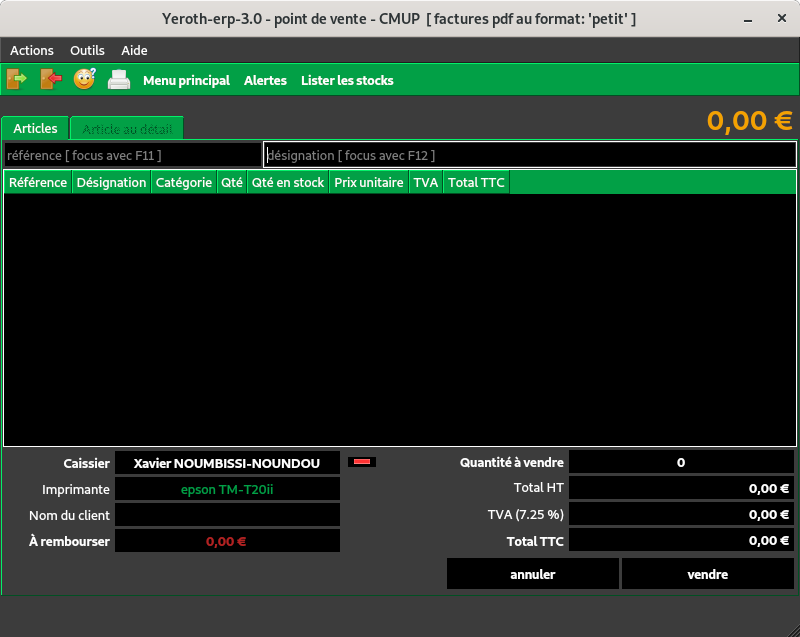
\includegraphics[scale=0.63]{images/yeren-fenetre-caissier.png}
	\caption{La fen\^etre pour vendre les articles.}
	\label{fig:fenetre-vendre}
\end{figure}

Le tableau o\`u sont affich\'es les articles \`a vendre
a les colones suivantes:
\begin{enumerate}[1)]
	\item R\'ef\'erence
	\item D\'esignation
	\item P.U. (\textbf{Prix Unitaire})
	\item Qt\'e (\textbf{Quantit\'e})
	\item Qt\'e restante en stock (\textbf{Quantit\'e restante en stock})
	\item Total TTC (\textbf{Total Toute Taxes Comprise})	
	\item TVA (\textbf{Taxe sur la Valeur Ajout\'e}).
\end{enumerate}

\subsection{La strat\'egie de vente utilis\'ee}
\index{La strat\'egie de vente des articles}
\index{La strat\'egie de vente des stocks}

Le titre de la fen\^etre affiche la strat\'egie de vente
des stocks utilis\'ee. Dans la figure~\ref{fig:fenetre-vendre}
par exemple, la strat\'egie de vente utilis\'ee est
\cmup.

\newpage
%-----------------------------------------------------------

\nxsection{S\'electionner des articles
	\`a vendre}\label{sec:selectionner-articles-vendre}
\index{s\'electionner des articles \`a vendre}
\index{s\'electionner des stocks \`a vendre}

Il existe $2$ m\'ethodes pour s\'electionner des articles
\`a vendre:
\begin{itemize}[\mycheckmark{purplish}]
	\item \textcolor{purplish}{$\mathbf{1^{\text{\`ere}}}$ \textbf{m\'ethode}}\\
	S\'electionner les stocks des articles \`a vendre
	en entrant leur code bar dans le premier champs de texte
	de l'interface (voir figure~\ref{fig:yeren-vendre-choisir-stock-codebar})
	\begin{figure}[!htbp]
		\centering
		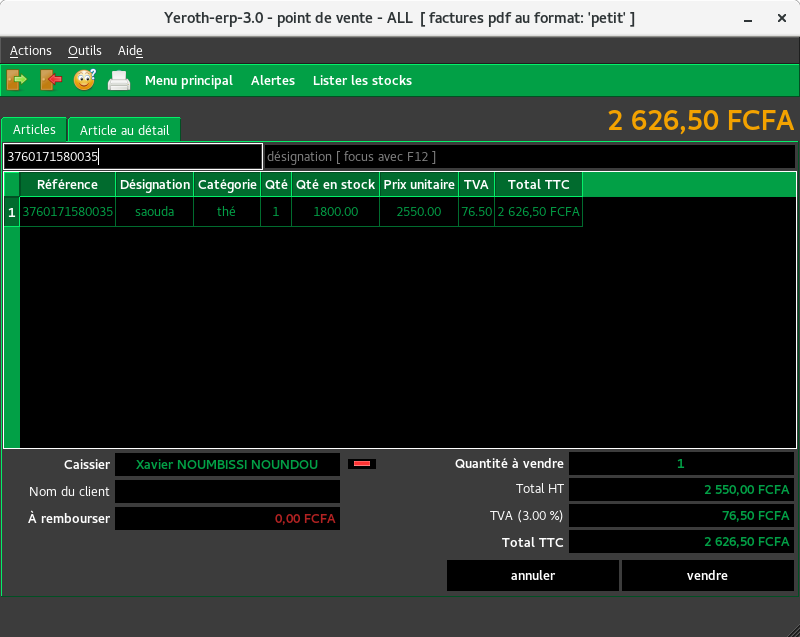
\includegraphics[scale=0.63]{images/yeren-vendre-choisir-stock-codebar.png}
		\caption{Le champs de texte pour
			ajouter les articles en utilisant leur code bar.}\label{fig:yeren-vendre-choisir-stock-codebar}
	\end{figure}
	
	\newpage
	\item \textcolor{purplish}{$\mathbf{2^{\text{\`eme}}}$ \textbf{m\'ethode}}\\
	S\'electionner les stocks des articles \`a vendre
	en entrant leur d\'esignation dans le deuxi\`eme
	champs de texte de l'interface
	(voir figure~\ref{fig:yeren-vendre-choisir-stock-designation}).
	\begin{figure}[!htbp]
		\centering
		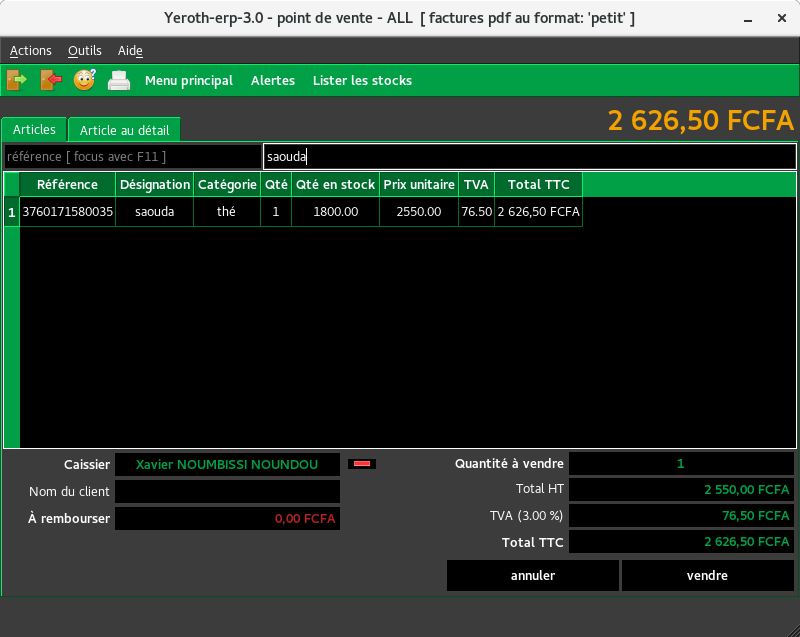
\includegraphics[scale=0.63]{images/yeren-vendre-choisir-stock-designation.png}
		\caption{Le champs de texte pour
			ajouter les articles en utilisant leur d\'esignation.}\label{fig:yeren-vendre-choisir-stock-designation}
	\end{figure}
\end{itemize}

\newpage

%----------------------------------------------------------- 

\nxsection{Afficher les d\'etails d'un article / stock
			s\'electionn\'e pour la vente}
\index{afficher les d\'etails d'un article \`a vendre}
\index{afficher les d\'etails d'un stock \`a vendre}

La figure~\ref{fig:yeren-vente-afficher-details-stock}
illustre les d\'etails du stock 'Saouda'.

Il existe deux m\'etodes pour voir les d\'etails
d'un stock s\'electionn\'e pour la vente:
\begin{itemize}[\mycheckmark{purplish}]
	\item \textcolor{purplish}{$\mathbf{1^{\text{\`ere}}}$ \textbf{m\'ethode}}\\
	Il suffit de cliquer deux fois sur n'importe quelle
	partie autre que '\textbf{Qt\'e}' de la ligne du
	stock s\'electionn\'e.\\
	
	\item \textcolor{purplish}{$\mathbf{2^{\text{\`eme}}}$ \textbf{m\'ethode}}\\
	Il suffit de cliquer sur l'onglet '\textbf{Article au d\'etail}'
	apr\`es la s\'election du stock.
\end{itemize}

%-----------------------------------------------------------
\newpage
\nxsection{Changer la quantit\'e \`a vendre
			d'un article / stock}\label{sec:changer-qte-vendre}
\index{changer la quantit\'e d'un article \`a vendre}
\index{changer la quantit\'e d'un stock \`a vendre}

Il existe deux m\'etodes pour changer la quantit\'e
d'articles d'un stock:
\begin{itemize}[\mycheckmark{purplish}]
	\item \textcolor{purplish}{$\mathbf{1^{\text{\`ere}}}$ \textbf{m\'ethode}}\\
	il faut cliquer sur l'\'el\'ement '\textbf{Qt\'e}'
	avec le bouton gauche de la souris, et ensuite changer la
	quantit\'e \`a vendre (voir figure~\ref{fig:yeren-vendre-qte-selectionner})
	\begin{figure}[!htbp]
		\centering
		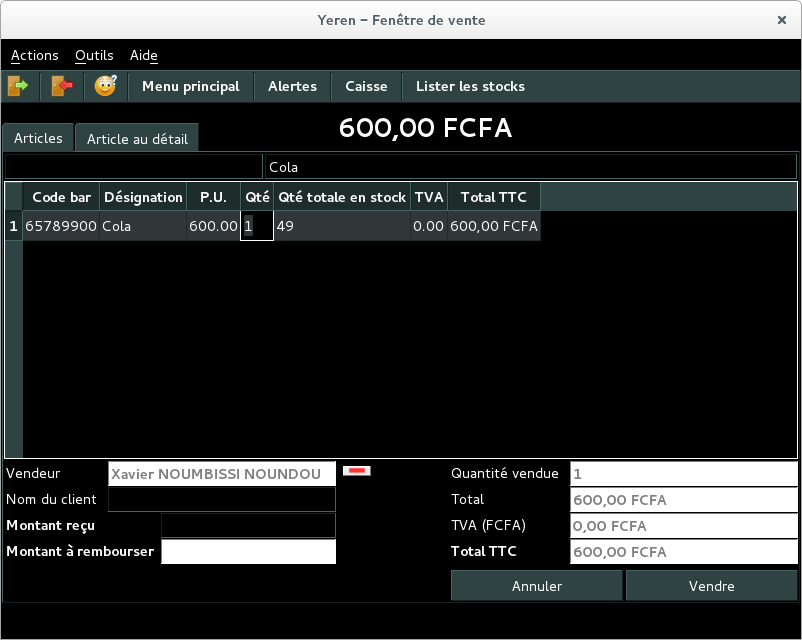
\includegraphics[scale=0.63]{images/yeren-vendre-qte-selectionner.png}
		\caption{L'\'el\'ement 'Qt\'e' s\'electionn\'e pour
			changer la quantit\'e d'articles 'Cola' \`a vendre.}\label{fig:yeren-vendre-qte-selectionner}
	\end{figure}
	\newpage
	
	\item \textcolor{purplish}{$\mathbf{2^{\text{\`eme}}}$ \textbf{m\'ethode}}\\
	il faut cliquer deux fois sur n'importe quel autre
	partie de la ligne du stock s\'electionn\'e, autre que 'Qt\'e'
	pour avoir acc\`es \`a une vue d\'etaill\'ee de ce stock.\\
	
	La vue de d\'etails du stock permet de changer
	la quantit\'e \`a vendre dans le champ de texte
	'\textbf{quantit\'e \`a vendre}'
	(voir figure~\ref{fig:yeren-vente-afficher-details-stock}).
	\begin{figure}[!htbp]
		\centering
		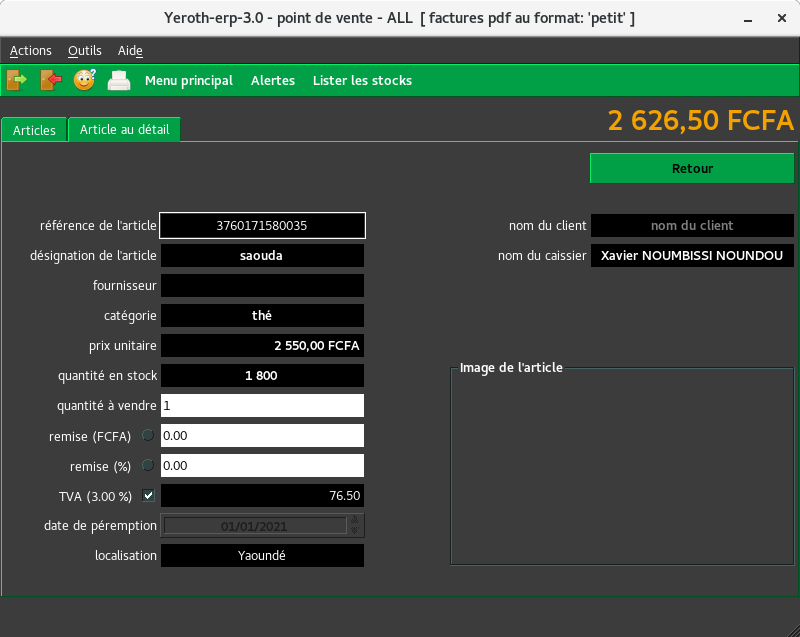
\includegraphics[scale=0.63]{images/yeren-vente-afficher-details-stock.png}
		\caption{Le champs de texte 'quantit\'e \`a vendre'
			permet de changer la quantit\'e \`a vendre d'un article.}
			\label{fig:yeren-vente-afficher-details-stock}
	\end{figure}
\end{itemize}

%-----------------------------------------------------------

\newpage
\nxsection{Appliquer une remise sur
			un article / stock \`a vendre}\label{sec:appliquer-remise-sur-article}
\index{appliquer un rabais sur un article}
\index{appliquer une remise sur un article}
\index{appliquer un rabais sur un stock}
\index{appliquer une remise sur un stock}

Voici la d\'emarche \`a suivre pour appliquer une remise
sur le prix unitaire d'un article \`a vendre:

\begin{enumerate}[1)]
	\item S\'electionner l'article \`a vendre (voir section~\ref{sec:selectionner-articles-vendre})
	\item ouvrer la vue de d\'etails de l'article auquel
		vous souhaitez appliquer une remise
		
	\item appliquer la remise en FCFA ou en pourcentage,
		en choisissant respectivement les bouton de radio
		\bouton{remise (FCFA)} ou \bouton{remise (\%)}, et
		en entrant le montant ou le pourcentage de remise
		\`a appliquer. (voir figure~\ref{fig:yeren-vente-afficher-details-stock})
		
	\item vous pouvez ensuite conclure la vente (voir section~\ref{sec:conclure-une-vente}).
\end{enumerate} 

%-----------------------------------------------------------

\nxsection{Modifier la TVA sur un article \`a vendre}\label{sec:modifier-TVA-article}
\index{ajouter la TVA sur le co\^ut d'un article}
\index{supprimer la TVA sur co\^ut d'un article}

Voici la d\'emarche \`a suivre pour retirer ou ajouter
la TVA sur un article \`a vendre:

\begin{enumerate}[1)]
	\item S\'electionner l'article \`a vendre (voir section~\ref{sec:selectionner-articles-vendre})
	\item ouvrer la vue de d\'etails de l'article auquel
	vous souhaitez appliquer une remise
	
	\item retirer ou ajouter la TVA en cochant le 'check box'
	TVA (voir figure~\ref{fig:yeren-vente-afficher-details-stock}).
	
	\item vous pouvez ensuite conclure la vente (voir section~\ref{sec:conclure-une-vente}).
\end{enumerate} 

%-----------------------------------------------------------
\newpage
\nxsection{Supprimer un article de la liste des articles \`a vendre}
\index{supprimer un article de la liste des articles \`a vendre}

\begin{figure}[!htbp]
	\centering
	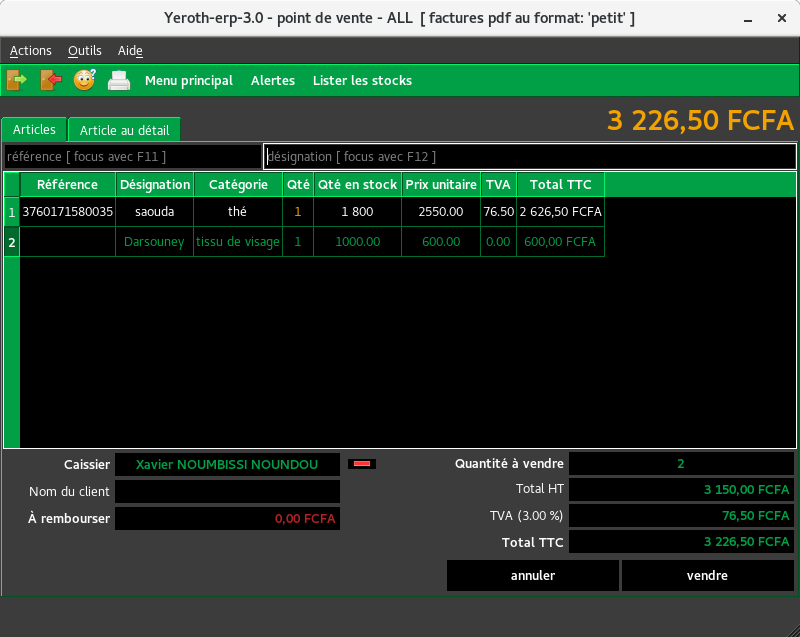
\includegraphics[scale=0.63]{images/yeren-vendre-supprimer-article.png}
	\caption{Le bouton rouge sert \`a supprimer un article
		de la liste des articles \`a vendre.}
	\label{fig:yeren-vendre-supprimer-article}
\end{figure}

Il suffit de s\'electionner la ligne de l'article \`a vendre,
et ensuite cliquer sur le petit bouton rouge qui se trouve
juste apr\`es le champs de texte '\textbf{Caissier}'.

Ce bouton rouge est illustr\'e dans la figure~\ref{fig:yeren-vendre-supprimer-article},
juste apr\`es le champs de texte '\textbf{Caissier}'.
	
%-----------------------------------------------------------
\newpage
\nxsection{Vendre \`a un client divers}\label{sec:vendre-client-divers}
\index{vendre \`a un client divers}

Il suffit de laisser le champs de texte '\textbf{Nom du client}'
vide lors de la vente.

%-----------------------------------------------------------

\nxsection{Vendre \`a un client nomm\'e}\label{sec:vendre-client-nomme}
\index{vendre \`a un client nomm\'e}

Il suffit de saisir le nom du client dans le champs de
texte '\textbf{Nom du client}'.

\begin{figure}[!htbp]
	\centering
	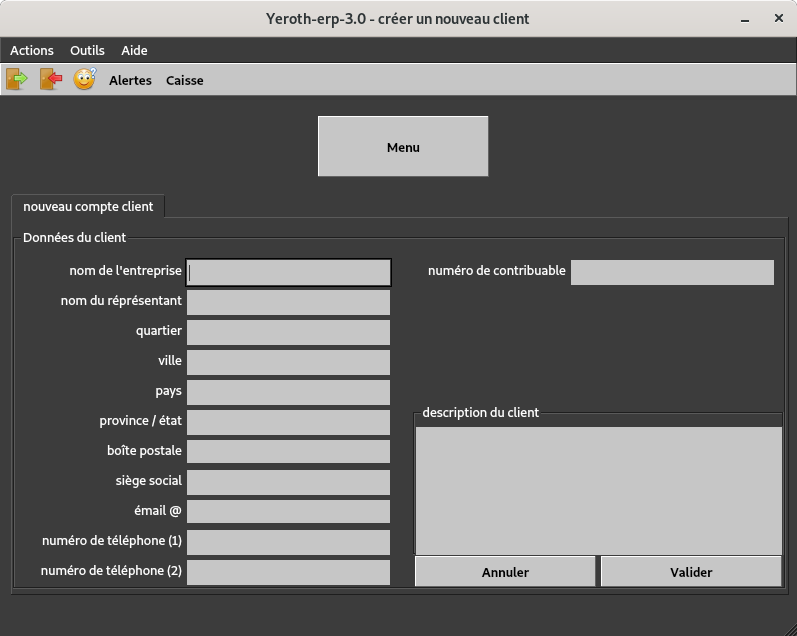
\includegraphics[scale=0.63]{images/yeren-vente-creer-nouveau-client.png}
	\caption{La fen\^etre de la cr\'eation d'un nouveau compte
		client \`a partir de l'interface de vente.}
	\label{fig:yeren-vente-creer-nouveau-client}
\end{figure}

Si le nom du client n'appara\^it pas dans la liste
sugg\'er\'ee, l'utilisateur doit s\'electionner le texte
'\textbf{nouveau client (*)}' (dans la liste sugg\'er'ee).
L'utilisateur sera alors conduit \`a la fen\^etre
pour cr\'eer un nouveau compte client
(figure~\ref{fig:yeren-vente-creer-nouveau-client}).

%-----------------------------------------------------------

\nxsection{Annuler une vente en cours}
\index{annuler une vente en cours}

Il suffit de cliquer sur le bouton \bouton{Annuler} pour annuler
une vente en cours.

%-----------------------------------------------------------

\nxsection{Conclure une vente}\label{sec:conclure-une-vente}
\index{conclure une vente}

Voici la d\'emarche \`a suivre pour conclure une vente:

\begin{enumerate}[1)]
	\item s\'electionner les articles \`a vendre
	(voir section~\ref{sec:selectionner-articles-vendre})
	
	\item entrer les quantit\'es \`a vendre 
	(voir section~\ref{sec:changer-qte-vendre})
	
	\item s'il y'a lieu, appliquer des remises ou modifier
	la TVA (voir section~\ref{sec:appliquer-remise-sur-article})
	
	\item enfin, retourner \`a la fen\^etre titr\'ee
	'\textbf{Yeren - Fen\^etre de la vente'} et
	presser sur le bouton \bouton{Vendre}
	(voir figure~\ref{fig:yeren-vendre-supprimer-article}).
\end{enumerate}

%-----------------------------------------------------------
\nxsection{Imprimer la facture \`a la suite d'une vente}
\index{imprimer la facture \`a la suite d'une vente}
\index{un exemple de facture}

\begin{figure}[!htbp]
	\centering
	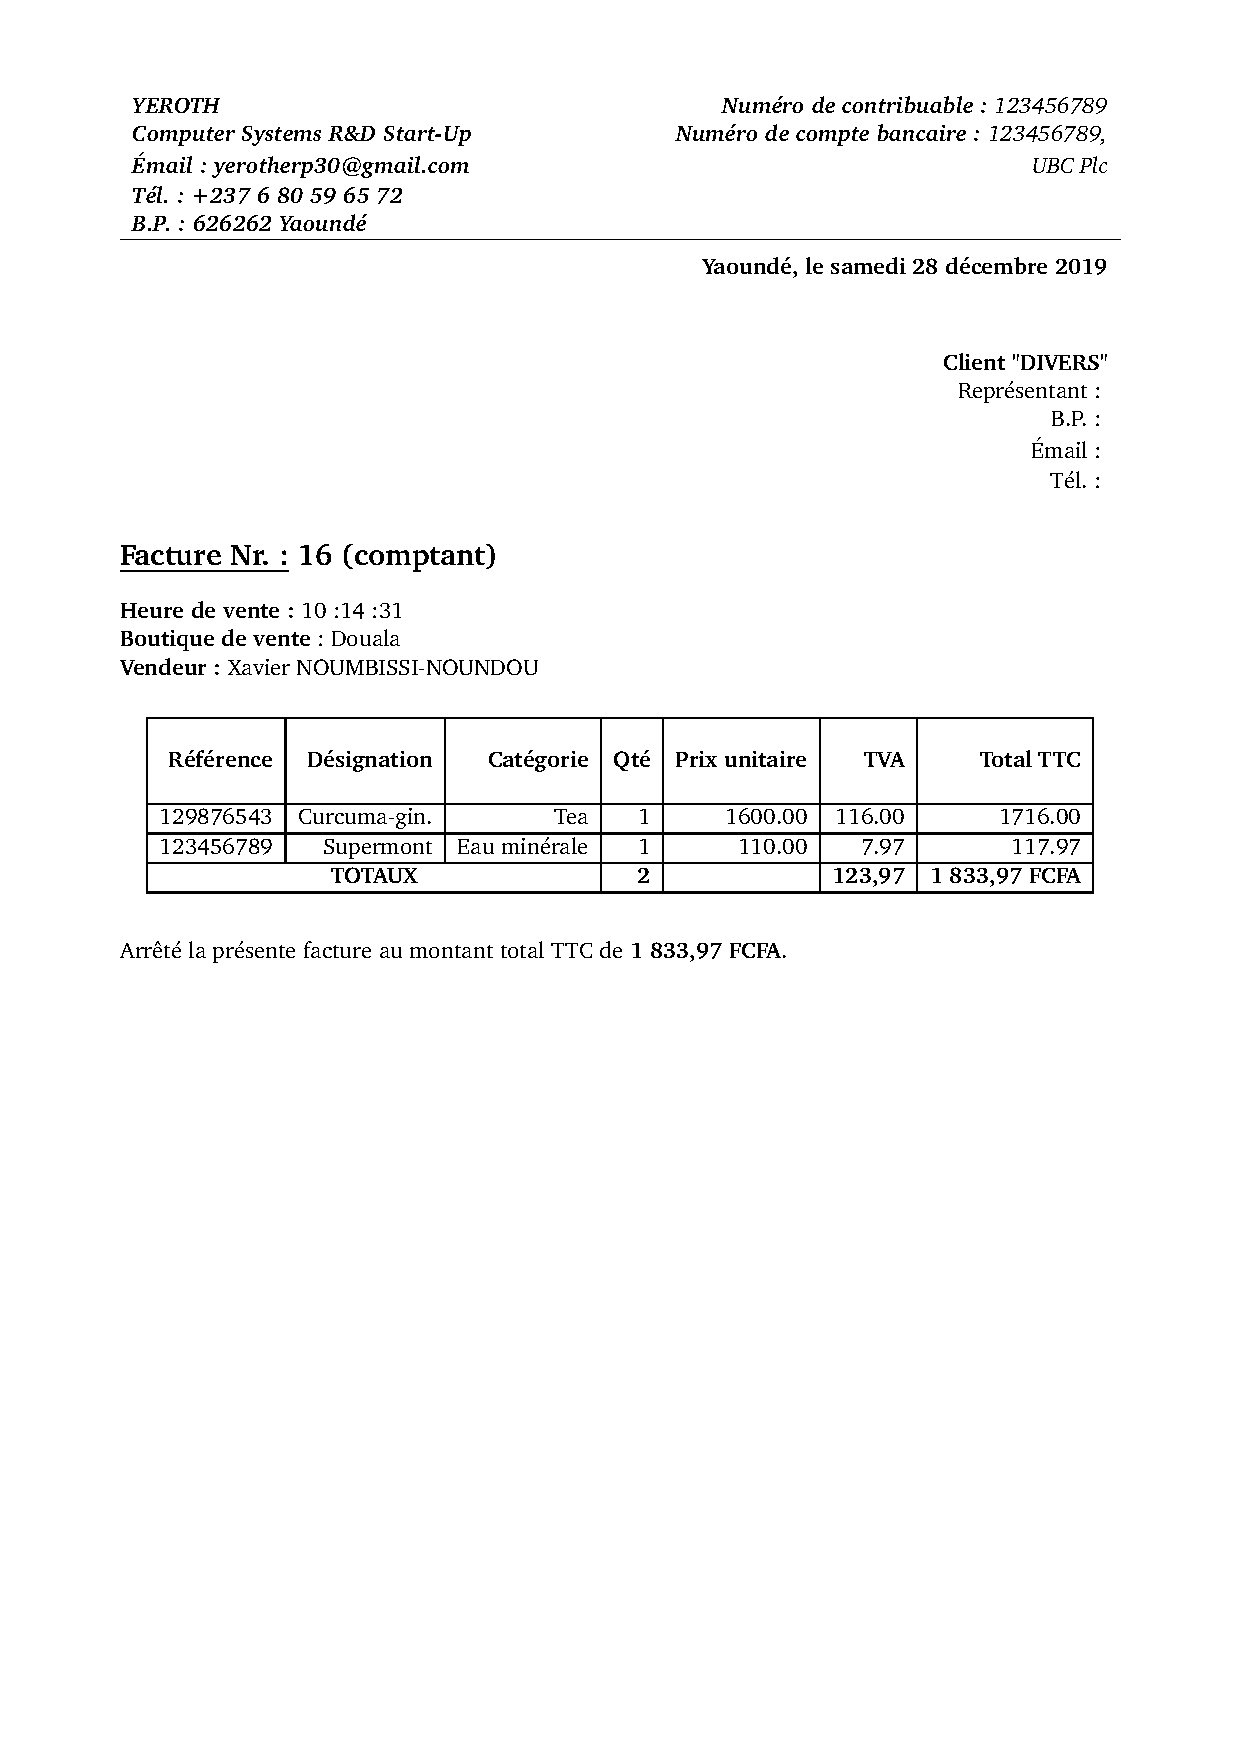
\includegraphics[scale=0.75]{images/yeren-facture-grand-2017-06-13.pdf}
	\caption{Une facture g\'en\'er\'ee \`a la suite d'une vente.}
	\label{fig:yeren-vendre-facture}
\end{figure}

Une facture au format PDF est automatiquement
g\'en\'erer, juste apr\`es qu'une vente soit effectu\'ee.
La figure~\ref{fig:yeren-vendre-facture} illustre un
exemple de facture.

%----------------------------------------------------------- 

\nxsection{Imprimer un exemple de facture au format
	PDF avant de conclure une vente}
\index{un exemple de facture au format PDF}
\index{imprimer un exemple de facture au format PDF}

\begin{figure}[!htbp]
	\centering
	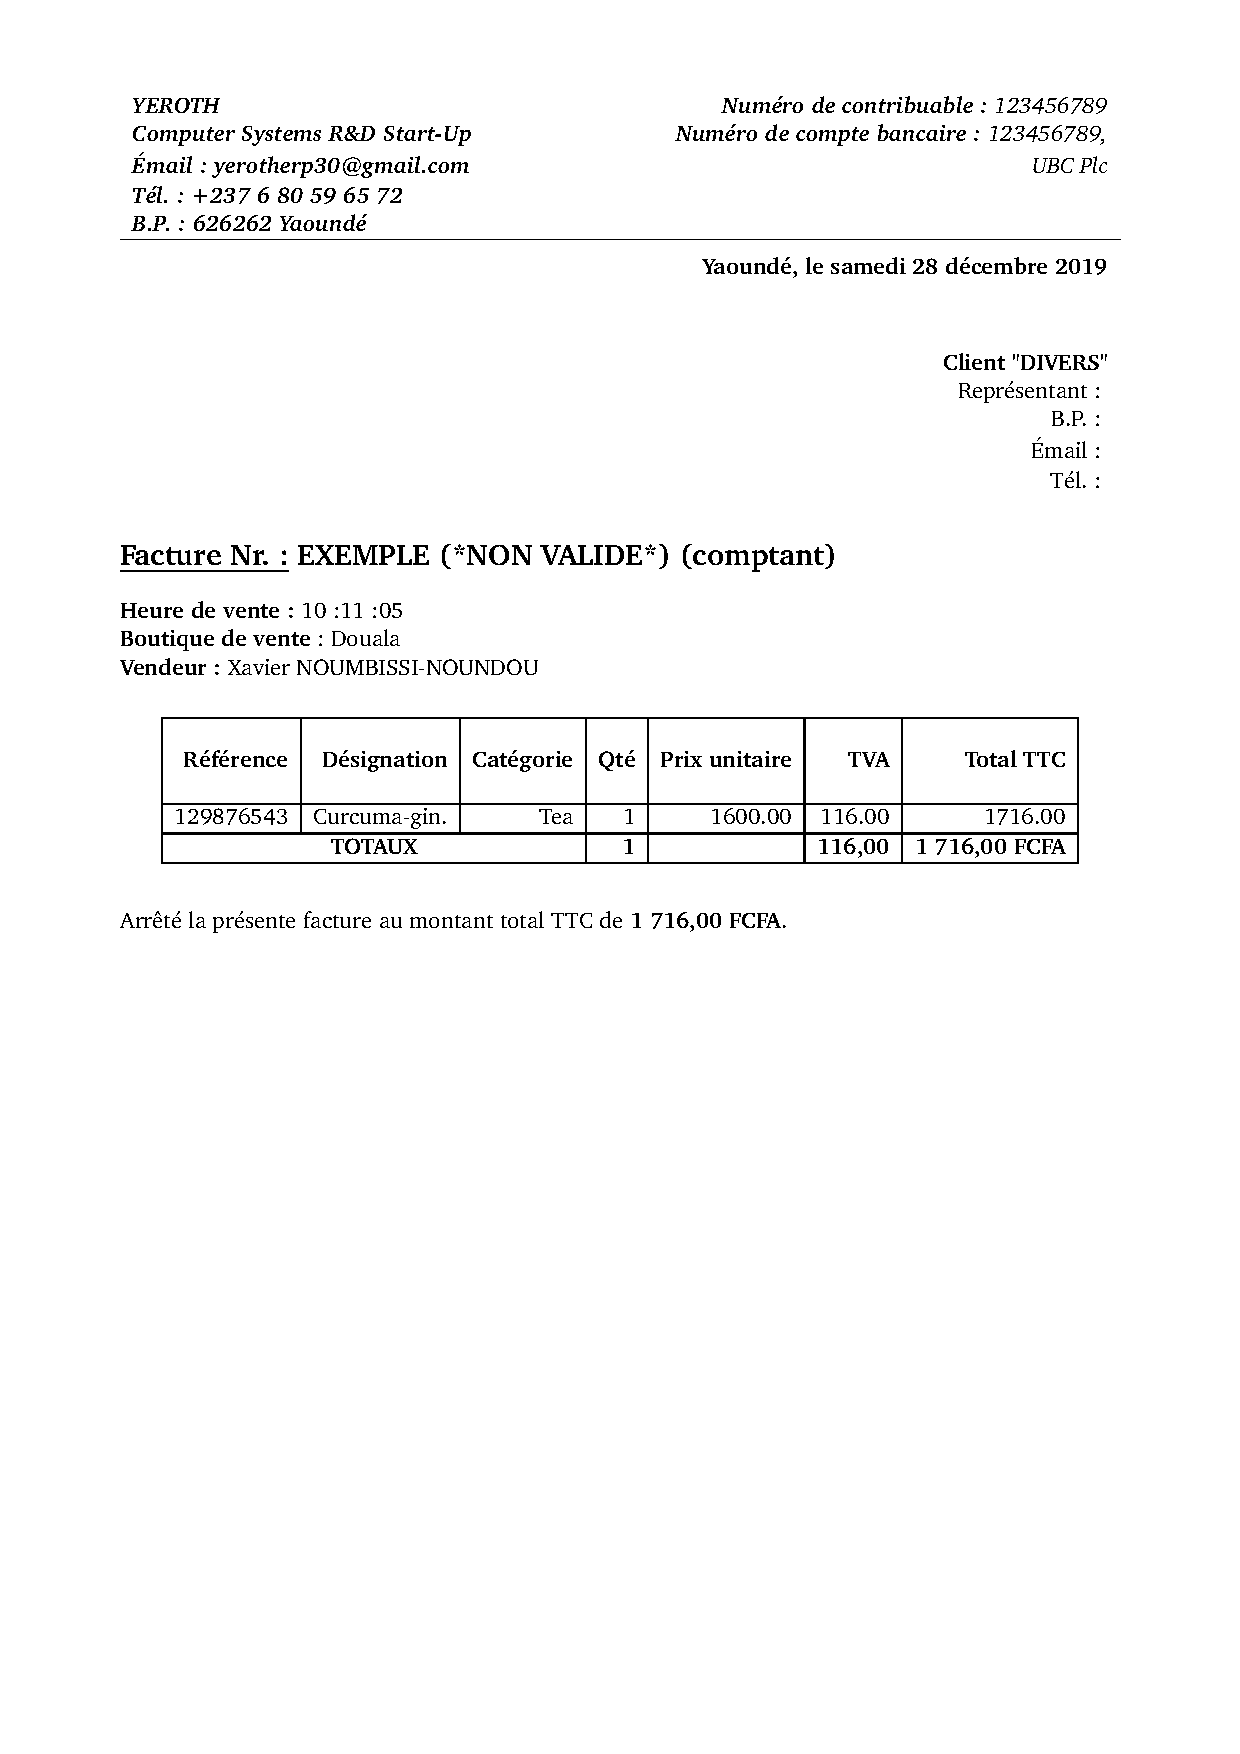
\includegraphics[scale=0.75]{images/yeren-exemple-facture-grand-2017-06-13.pdf}
	\caption{Une facture proforma g\'en\'er\'ee avant de conclure une vente.}
	\label{fig:yeren-vendre-facture-proforma}
\end{figure}

Il existe deux m\'ethodes pour imprimer une facture
proforma avant de conclure la vente \'eventuelle des articles
pr\'esents dans le tableau qui appara\^it dans la fen\^etre
titr\'ee '\textbf{Yeren - Fen\^etre de la vente}'.

\begin{itemize}[\mycheckmark{purplish}]
	\item \textcolor{purplish}{$\mathbf{1^{\text{\`ere}}}$ \textbf{m\'ethode}}\\
		Cliquer sur le lien '\textbf{Imprimer la facture (proforma)}'
		qui se trouve dans le menu d\'eroulant '\textbf{Outils}'\\

	\item \textcolor{purplish}{$\mathbf{2^{\text{\`eme}}}$ \textbf{m\'ethode}}\\
		Presser simultan\'ement les boutons \bouton{CTRL}
		et \bouton{P} de votre clavier.
\end{itemize}

Une facture proforma au format PDF est alors g\'en\'er\'ee. Un
exemple de facture proforma est illustr\'e dans la
figure~\ref{fig:yeren-vendre-facture-proforma}.
